\documentclass{standalone}
\usepackage{fontspec}
\usepackage{tikz}
\usetikzlibrary{arrows.meta,calc,positioning}
\begin{document}
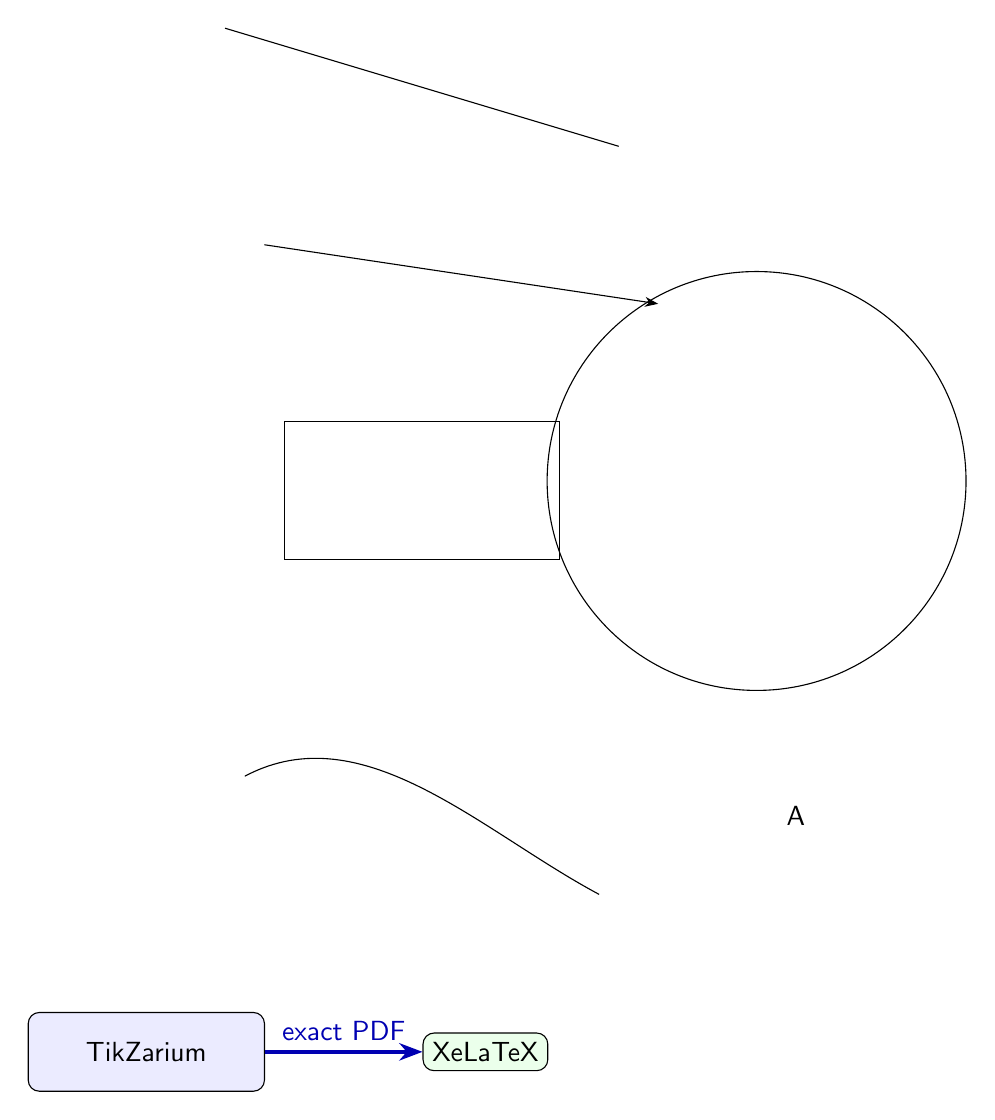
\begin{tikzpicture}[>=Stealth, every node/.style={font=\sffamily}]
  \node[draw,rounded corners,fill=blue!8,minimum width=3cm,minimum height=1cm] (A) {TikZarium};
  \node[draw,rounded corners,fill=green!8,right=2cm of A] (B) {XeLaTeX};
  \draw[->,very thick,blue!70!black] (A) -- node[above] {exact PDF} (B);
  \draw (1.00cm,13.00cm) -- (6.00cm,11.50cm); % tikzarium:n1:[2,1,"line",{"end_x":"6.00cm","end_y":"11.50cm","start_x":"1.00cm","start_y":"13.00cm"}]
  \draw[-{Stealth}] (1.50cm,10.25cm) -- (6.50cm,9.50cm); % tikzarium:n1:[2,2,"arrow",{"end_x":"6.50cm","end_y":"9.50cm","start_x":"1.50cm","start_y":"10.25cm","tip":"Stealth"}]
  \draw (1.75cm,8.00cm) rectangle (5.25cm,6.25cm); % tikzarium:n1:[2,3,"rectangle",{"end_x":"5.25cm","end_y":"6.25cm","start_x":"1.75cm","start_y":"8.00cm"}]
  \draw (7.75cm,7.25cm) circle[radius=2.66cm]; % tikzarium:n1:[2,4,"circle",{"center_x":"7.75cm","center_y":"7.25cm","radius":"2.66cm"}]
  \node at (8.25cm,3.00cm) {A}; % tikzarium:n1:[2,5,"node",{"content":"A","mode":"text","x":"8.25cm","y":"3.00cm"}]
  \draw (1.25cm,3.50cm) .. controls (2.75cm,4.30cm) and (4.25cm,2.80cm) .. (5.75cm,2.00cm); % tikzarium:n1:[2,6,"cubic",{"control1_x":"2.75cm","control1_y":"4.30cm","control2_x":"4.25cm","control2_y":"2.80cm","end_x":"5.75cm","end_y":"2.00cm","start_x":"1.25cm","start_y":"3.50cm"}]
\end{tikzpicture}
\end{document}
